\section{User Management}
%%%%%%%%%%%%%%%%%%%%%%%%%%%%%%%%%%%%%%%%%%%%%%%%%%%%%%%%%%%%%%%%%%%%%%%%%%%% 
%%%%%%%%%%%%%%%%%%%%%%%%%%%%%%%%%%%%%%%%%%%%%%%%%%%%%%%%%%%%%%%%%%%%%%%%%%%% 
%%%%%%%%%%%%%%%%%%%%%%%%%%%%%%%%%%%%%%%%%%%%%%%%%%%%%%%%%%%%%%%%%%%%%%%%%%%% 
%%%%%%%%%%%%%%%%%%%%%%%%%%%%%%%%%%%%%%%%%%%%%%%%%%%%%%%%%%%%%%%%%%%%%%%%%%%% 
\begin{frame}[t,fragile]{Adding an user to the system}
  % ------------------------------------------------------


  \begin{block}{Adding users with the \alert{\texttt{adduser}} command}
    {\footnotesize
Easy way to add users to the system with a console interactive application. \\Syntax is \alert{\texttt{adduser} \emph{username}} and the new user's password is defined on the fly.}

{\scriptsize
  \begin{lstlisting}
$ sudo adduser bobby
[sudo] password for alice: 
...
Enter new UNIX password: 
Retype new UNIX password: 
passwd: password updated successfully
Changing the user information for bobby
Enter the new value, or press ENTER for the default
	Full Name []: Bobby Doe
........
Is the information correct? [Y/n] y
$ 
  \end{lstlisting}
}
    {\footnotesize
If the new user is expected to have administration privileges (e.g.\ use of \texttt{sudo})  it has to be added to the \texttt{admin} group. This can be done with the command \\\alert{\texttt{adduser } \emph{username} \texttt{sudo}}.}

  \end{block}
  
%%%%%%%%%%%%%%%%%%%%%%%%%%%%%%%%%%%%%%%%%%%%%%%%%%%%%%%%%%%%%%%%%%%%%%%%%%%%%%%%%%
\note{
{\tiny

Notes Module V
}
}
\end{frame}
%%%%%%%%%%%%%%%%%%%%%%%%%%%%%%%%%%%%%%%%%%%%%%%%%%%%%%%%%%%%%%%%%%%%%%%%%%%% 
%%%%%%%%%%%%%%%%%%%%%%%%%%%%%%%%%%%%%%%%%%%%%%%%%%%%%%%%%%%%%%%%%%%%%%%%%%%% 
\begin{frame}[t,fragile]{Removing an user from the system}
  % ------------------------------------------------------


  \begin{block}{Removing users with the \alert{\texttt{deluser}} command}
    {\footnotesize
A user removal is accomplished with the command: \alert{\texttt{deluser} \emph{username}}\\ 
If the user home directory has to be deleted too then the option \texttt{{-}-remove-home} needs to be included. The similar command \alert{\texttt{delgroup}} is used to remove unwanted user groups.}

{\footnotesize
  \begin{lstlisting}
$ sudo deluser --remove-home bobby
[sudo] password for alice: 
Looking for files to backup/remove ...
Removing files ...
Removing user `bobby' ...
Warning: group `bobby' has no more members.
Done.
$ sudo delgroup bobby
The group `bobby' does not exist.
$ cat /etc/group | grep bobby
$ 
  \end{lstlisting}
}

  \end{block}
  
%%%%%%%%%%%%%%%%%%%%%%%%%%%%%%%%%%%%%%%%%%%%%%%%%%%%%%%%%%%%%%%%%%%%%%%%%%%%%%%%%%
\note{
{\tiny

Notes Module V
}
}
\end{frame}
%%%%%%%%%%%%%%%%%%%%%%%%%%%%%%%%%%%%%%%%%%%%%%%%%%%%%%%%%%%%%%%%%%%%%%%%%%%% 
%%%%%%%%%%%%%%%%%%%%%%%%%%%%%%%%%%%%%%%%%%%%%%%%%%%%%%%%%%%%%%%%%%%%%%%%%%%% 
%%%%%%%%%%%%%%%%%%%%%%%%%%%%%%%%%%%%%%%%%%%%%%%%%%%%%%%%%%%%%%%%%%%%%%%%%%%% 
%%%%%%%%%%%%%%%%%%%%%%%%%%%%%%%%%%%%%%%%%%%%%%%%%%%%%%%%%%%%%%%%%%%%%%%%%%%% 
\section{Basics of Private/Public Key Approach}
%%%%%%%%%%%%%%%%%%%%%%%%%%%%%%%%%%%%%%%%%%%%%%%%%%%%%%%%%%%%%%%%%%%%%%%%%%%% 
%%%%%%%%%%%%%%%%%%%%%%%%%%%%%%%%%%%%%%%%%%%%%%%%%%%%%%%%%%%%%%%%%%%%%%%%%%%% 
%%%%%%%%%%%%%%%%%%%%%%%%%%%%%%%%%%%%%%%%%%%%%%%%%%%%%%%%%%%%%%%%%%%%%%%%%%%% 
%%%%%%%%%%%%%%%%%%%%%%%%%%%%%%%%%%%%%%%%%%%%%%%%%%%%%%%%%%%%%%%%%%%%%%%%%%%% 
%%%%%%%%%%%%%%%%%%%%%%%%%%%%%%%%%%%%%%%%%%%%%%%%%%%%%%%%%%%%%%%%%%%%%%%%%%%% 
%%%%%%%%%%%%%%%%%%%%%%%%%%%%%%%%%%%%%%%%%%%%%%%%%%%%%%%%%%%%%%%%%%%%%%%%%%%%
\begin{frame}[t,fragile]{What is the private/public key approach?}
  % ------------------------------------------------------
  \begin{block}{The \alert{private} and \alert{public} keys}
    {\footnotesize
Every digital certificate has a pair of associated cryptographic
keys. This pair of keys consists of a \textbf{private} key and a \textbf{public} key. 

\vspace{0.25cm}
A \textbf{public} key is part of the owner's digital certificate and \emph{it is available for anyone to use}. A \textbf{private} key, however, is protected by and \emph{available only to the owner of the key}. This limited access ensures that communications that use the key are kept secure.

\vspace{0.25cm}
The owner of a certificate can use these keys to take advantage of the
cryptographic security features that the keys provide. For example,
the certificate owner can use a certificate's private key to ``sign''
and encrypt data sent between users and servers, such as messages,
documents, and code objects. The recipient of the signed object can
then use the public key contained in the signer's certificate to
decrypt the signature. Such digital signatures ensure the reliability
of an object's origin and provide a means of checking the integrity of
the object.
}
  \end{block}
  
%%%%%%%%%%%%%%%%%%%%%%%%%%%%%%%%%%%%%%%%%%%%%%%%%%%%%%%%%%%%%%%%%%%%%%%%%%%%%%%%%%
\note{
{\tiny

Notes Module V
}
}
\end{frame}
%%%%%%%%%%%%%%%%%%%%%%%%%%%%%%%%%%%%%%%%%%%%%%%%%%%%%%%%%%%%%%%%%%%%%%%%%%%% 
%%%%%%%%%%%%%%%%%%%%%%%%%%%%%%%%%%%%%%%%%%%%%%%%%%%%%%%%%%%%%%%%%%%%%%%%%%%%
%%%%%%%%%%%%%%%%%%%%%%%%%%%%%%%%%%%%%%%%%%%%%%%%%%%%%%%%%%%%%%%%%%%%%%%%%%%% 
%%%%%%%%%%%%%%%%%%%%%%%%%%%%%%%%%%%%%%%%%%%%%%%%%%%%%%%%%%%%%%%%%%%%%%%%%%%% 
%%%%%%%%%%%%%%%%%%%%%%%%%%%%%%%%%%%%%%%%%%%%%%%%%%%%%%%%%%%%%%%%%%%%%%%%%%%% 
%%%%%%%%%%%%%%%%%%%%%%%%%%%%%%%%%%%%%%%%%%%%%%%%%%%%%%%%%%%%%%%%%%%%%%%%%%%% 
\section{Securely Login in Remote Systems}
%%%%%%%%%%%%%%%%%%%%%%%%%%%%%%%%%%%%%%%%%%%%%%%%%%%%%%%%%%%%%%%%%%%%%%%%%%%% 
%%%%%%%%%%%%%%%%%%%%%%%%%%%%%%%%%%%%%%%%%%%%%%%%%%%%%%%%%%%%%%%%%%%%%%%%%%%% 
%%%%%%%%%%%%%%%%%%%%%%%%%%%%%%%%%%%%%%%%%%%%%%%%%%%%%%%%%%%%%%%%%%%%%%%%%%%% 
%%%%%%%%%%%%%%%%%%%%%%%%%%%%%%%%%%%%%%%%%%%%%%%%%%%%%%%%%%%%%%%%%%%%%%%%%%%% 
%%%%%%%%%%%%%%%%%%%%%%%%%%%%%%%%%%%%%%%%%%%%%%%%%%%%%%%%%%%%%%%%%%%%%%%%%%%% 
%%%%%%%%%%%%%%%%%%%%%%%%%%%%%%%%%%%%%%%%%%%%%%%%%%%%%%%%%%%%%%%%%%%%%%%%%%%%
\begin{frame}[t,fragile]{Secure login in remote systems}
  % ------------------------------------------------------
  \begin{block}{Fundamentals of the \alert{\texttt{ssh}} command}
    {\footnotesize
 The command \alert{\texttt{ssh}} is a powerful tool that allows the remote login in systems. After login with \texttt{\alert{ssh}} we can interact with the remote system via the \texttt{bash} shell as we do in the local system. 

 Let's imagine that we are currently working as username \texttt{\alert{bob}} in a local system with hostname \texttt{\alert{HAL}} and we want to log into a different system whose hostname is \texttt{\alert{EARTH}} and where our hostname is \texttt{\alert{bobby}}. 

  \begin{columns}
      \column{.5\textwidth}
The  \texttt{ssh} program allows to work remotely in a safe way encrypting the data using a \emph{public/private keypair}.
      \column{.5\textwidth}
\begin{center}
% \onslide*{2}{
% \includegraphics[angle=0,width=5cm]{./Figs/Diagram1.eps}}
%\onslide*{3}{
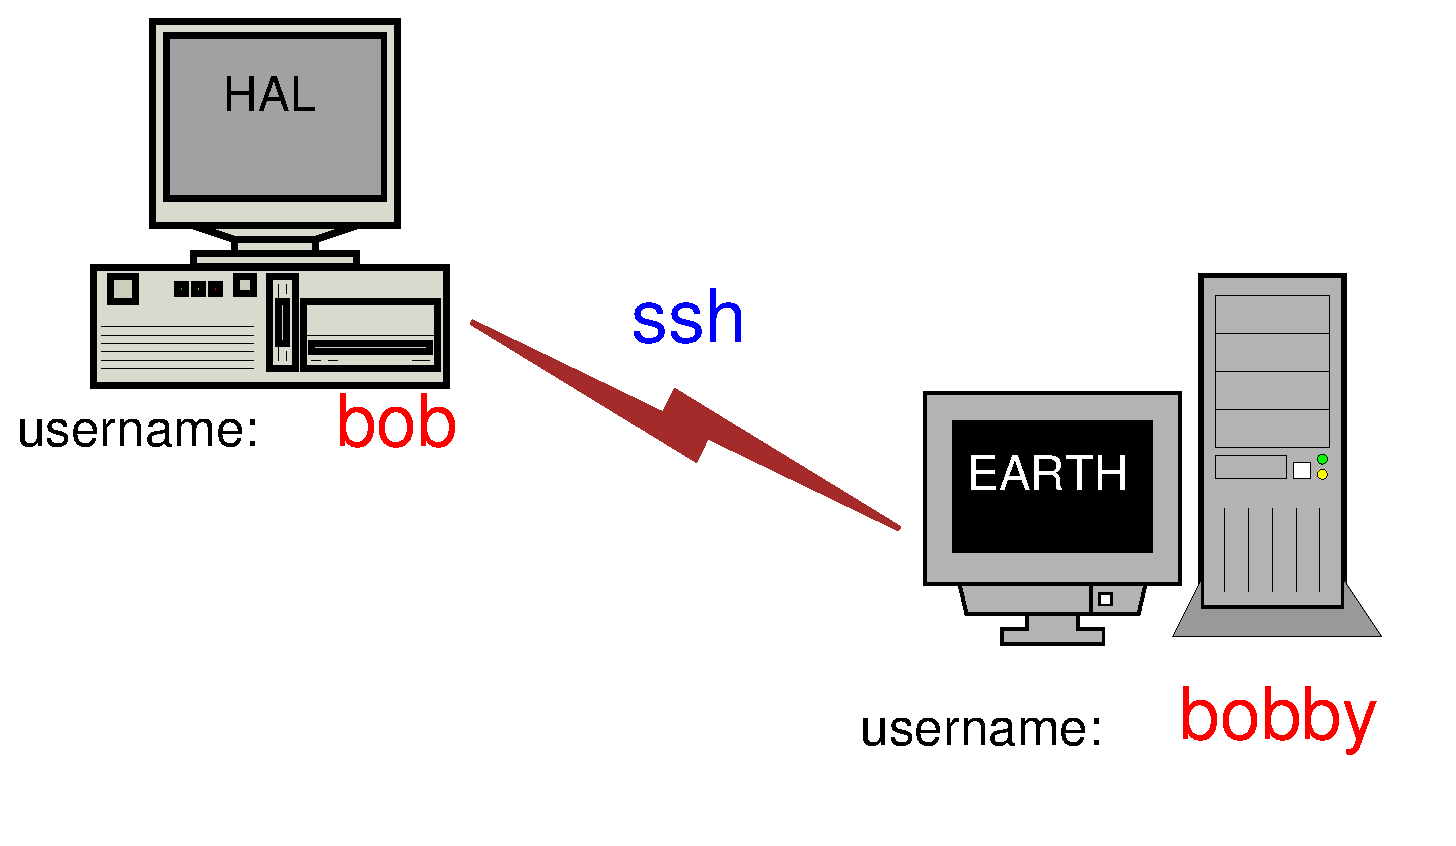
\includegraphics[angle=0,width=5cm]{./Figs/Diagram2.eps}%}
\end{center}
\end{columns}
}
  \end{block}
  
%%%%%%%%%%%%%%%%%%%%%%%%%%%%%%%%%%%%%%%%%%%%%%%%%%%%%%%%%%%%%%%%%%%%%%%%%%%%%%%%%%
\note{
{\tiny

Notes Module V
}
}
\end{frame}
%%%%%%%%%%%%%%%%%%%%%%%%%%%%%%%%%%%%%%%%%%%%%%%%%%%%%%%%%%%%%%%%%%%%%%%%%%%% 
%%%%%%%%%%%%%%%%%%%%%%%%%%%%%%%%%%%%%%%%%%%%%%%%%%%%%%%%%%%%%%%%%%%%%%%%%%%% 
\begin{frame}[t,fragile]{Using \alert{\texttt{ssh}}}
  % ------------------------------------------------------


  \begin{block}{Basic command syntax: \alert{\texttt{ssh} \emph{username}@\emph{hostname}}}
    {\footnotesize The first time that a computer is accessed by \texttt{ssh} its public key has to be acknowledged (more details later).}
{\scriptsize
  \begin{lstlisting}
bob@hal:~$ ssh bobby@earth
The authenticity of host 'earth (192.168.1.50)' can't be established.
RSA key fingerprint is 2d:f4:d4:4d:2b:b5:ad:23:0c:f2:db:16:1c:07:27:c1.
Are you sure you want to continue connecting (yes/no)? yes 
Warning: Permanently added 'earth' (RSA) to the list of known hosts.
bobby@earth's password: 
Welcome to Ubuntu 12.04.1 LTS (GNU/Linux 3.2.0-33-generic i686)
Last login: Sun Nov 18 11:18:24 2012 from nostromo
bobby@earth:~$ 
  \end{lstlisting}
}

{\footnotesize\textbf{(a)} In order to be able to login into a computer the package \texttt{openssh-server} has to be installed.\\
\textbf{(b)} The syntax to export the X windows is: 
\texttt{\alert{ssh -X} \emph{\alert{username@computer}}}\\
\textbf{(c)} To close the session use  \texttt{\alert{exit}} or \texttt{CTRL-D}.
}
  \end{block}
  
%%%%%%%%%%%%%%%%%%%%%%%%%%%%%%%%%%%%%%%%%%%%%%%%%%%%%%%%%%%%%%%%%%%%%%%%%%%%%%%%%%
\note{
{\tiny

Notes Module V
}
}
\end{frame}
%%%%%%%%%%%%%%%%%%%%%%%%%%%%%%%%%%%%%%%%%%%%%%%%%%%%%%%%%%%%%%%%%%%%%%%%%%%% 
%%%%%%%%%%%%%%%%%%%%%%%%%%%%%%%%%%%%%%%%%%%%%%%%%%%%%%%%%%%%%%%%%%%%%%%%%%%% 
\begin{frame}[t,fragile]{Running commands in remote systems}
  % ------------------------------------------------------
  \begin{block}{Remote command execution with \alert{\texttt{ssh}}}
    {\footnotesize
The command \alert{\texttt{ssh}} also allows to execute a command in a remote system, passing data streams to and receiving data streams from this command. 

As in the previous example, we are currently working as username \texttt{bob} in a local system with hostname \texttt{HAL}. Now we want to run \texttt{df -h} in a different system whose hostname is \texttt{EARTH} and where our hostname is \texttt{bobby}, appending the output to a file called \texttt{system\_df\_output.dat}. 

      \begin{center}
        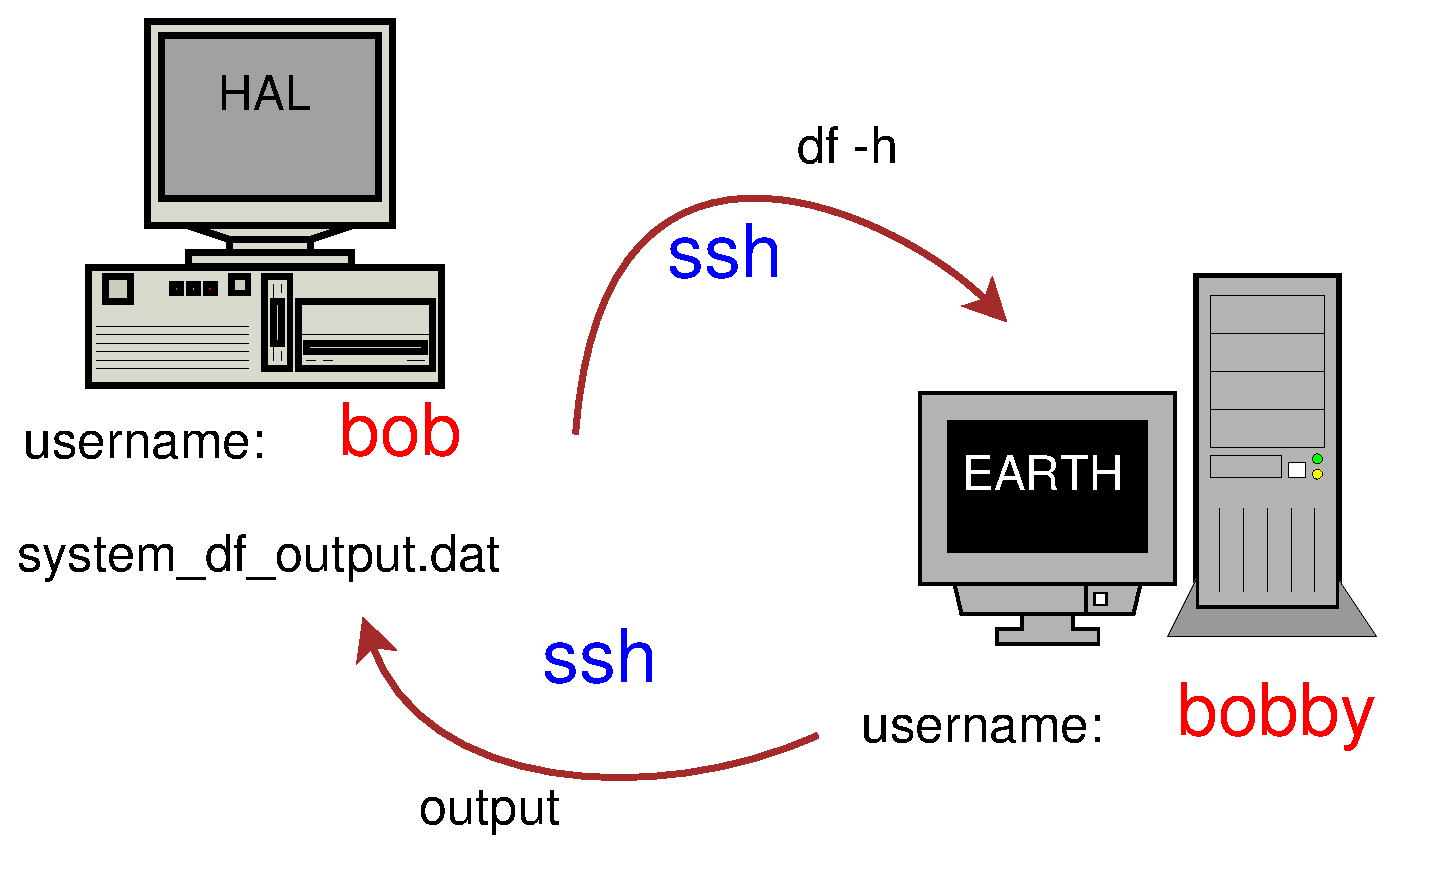
\includegraphics[angle=0,width=5cm]{./Figs/Diagram6.eps}%}
      \end{center}
    }
  \end{block}
  
%%%%%%%%%%%%%%%%%%%%%%%%%%%%%%%%%%%%%%%%%%%%%%%%%%%%%%%%%%%%%%%%%%%%%%%%%%%%%%%%%%
\note{
{\tiny

Notes Module V
}
}
\end{frame}
%%%%%%%%%%%%%%%%%%%%%%%%%%%%%%%%%%%%%%%%%%%%%%%%%%%%%%%%%%%%%%%%%%%%%%%%%%%% 
%%%%%%%%%%%%%%%%%%%%%%%%%%%%%%%%%%%%%%%%%%%%%%%%%%%%%%%%%%%%%%%%%%%%%%%%%%%% 
\begin{frame}[t,fragile]{Remote commands with \alert{\texttt{ssh}}}
  % ------------------------------------------------------


  \begin{block}{Basic command syntax: \alert{\texttt{ssh} \emph{username}@\emph{hostname} \emph{command}}}
    {\footnotesize 
  \begin{lstlisting}
bob@hal:~$ ssh bobby@earth "df -h" >> system_df_output.dat
bob@hal:~$ tail system_df_output.dat
Filesystem            Size  Used Avail Use% Mounted on
/dev/sda2              35G   29G  4.3G  88% /
tmpfs                 628M   12K  628M   1% /lib/init/rw
udev                  623M  272K  623M   1% /dev
tmpfs                 628M  816K  627M   1% /dev/shm
/dev/sdc2             202G   15G  177G   8% /media/usb_disk
/dev/sdc1             391G   21G  370G   6% /media/MSDOS
/dev/sr1              354M  354M     0 100% /media/WD SmartWare
  \end{lstlisting}
}

{\footnotesize The standard input can also be sent to \texttt{\alert{ssh}}}
    {\scriptsize 
  \begin{lstlisting}
bob@hal:~$ echo "Seems magic..." | ssh bobby@earth "cat > magic.dat"
Password:
bob@hal:~$ 
  \end{lstlisting}
}

  \end{block}
  
%%%%%%%%%%%%%%%%%%%%%%%%%%%%%%%%%%%%%%%%%%%%%%%%%%%%%%%%%%%%%%%%%%%%%%%%%%%%%%%%%%
\note{
{\tiny

Notes Module V
}
}
\end{frame}
%%%%%%%%%%%%%%%%%%%%%%%%%%%%%%%%%%%%%%%%%%%%%%%%%%%%%%%%%%%%%%%%%%%%%%%%%%%% 
%%%%%%%%%%%%%%%%%%%%%%%%%%%%%%%%%%%%%%%%%%%%%%%%%%%%%%%%%%%%%%%%%%%%%%%%%%%% 
%%%%%%%%%%%%%%%%%%%%%%%%%%%%%%%%%%%%%%%%%%%%%%%%%%%%%%%%%%%%%%%%%%%%%%%%%%%% 
%%%%%%%%%%%%%%%%%%%%%%%%%%%%%%%%%%%%%%%%%%%%%%%%%%%%%%%%%%%%%%%%%%%%%%%%%%%% 
%%%%%%%%%%%%%%%%%%%%%%%%%%%%%%%%%%%%%%%%%%%%%%%%%%%%%%%%%%%%%%%%%%%%%%%%%%%% 
%%%%%%%%%%%%%%%%%%%%%%%%%%%%%%%%%%%%%%%%%%%%%%%%%%%%%%%%%%%%%%%%%%%%%%%%%%%% 
\section{Secure Copy Within Remote Systems}
%%%%%%%%%%%%%%%%%%%%%%%%%%%%%%%%%%%%%%%%%%%%%%%%%%%%%%%%%%%%%%%%%%%%%%%%%%%% 
%%%%%%%%%%%%%%%%%%%%%%%%%%%%%%%%%%%%%%%%%%%%%%%%%%%%%%%%%%%%%%%%%%%%%%%%%%%% 
%%%%%%%%%%%%%%%%%%%%%%%%%%%%%%%%%%%%%%%%%%%%%%%%%%%%%%%%%%%%%%%%%%%%%%%%%%%% 
%%%%%%%%%%%%%%%%%%%%%%%%%%%%%%%%%%%%%%%%%%%%%%%%%%%%%%%%%%%%%%%%%%%%%%%%%%%% 
%%%%%%%%%%%%%%%%%%%%%%%%%%%%%%%%%%%%%%%%%%%%%%%%%%%%%%%%%%%%%%%%%%%%%%%%%%%% 
%%%%%%%%%%%%%%%%%%%%%%%%%%%%%%%%%%%%%%%%%%%%%%%%%%%%%%%%%%%%%%%%%%%%%%%%%%%%
\begin{frame}[t,fragile]{Secure file transfer to remote systems}
  % ------------------------------------------------------
  \begin{block}{Fundamentals of the \alert{\texttt{scp}} command}
    {\footnotesize
      The command \alert{\texttt{scp}}  allows to copy in a secure way files to and from remote systems. Let's imagine that we are currently working as username \texttt{\alert{bob}} in a local system with hostname \texttt{HAL} and we want to transfer some files to a different system whose hostname is \texttt{EARTH} and where our hostname is \texttt{\alert{bobby}}.  

  \begin{columns}
      \column{.5\textwidth}\texttt{\alert{scp}} allows to work remotely in a safe way encrypting the data using a \alert{public/private keypair}.

      \column{.5\textwidth}
\begin{center}
% \onslide*{2}{
% \includegraphics[angle=0,width=5cm]{./Figs/Diagram1.eps}}
%\onslide*{3}{
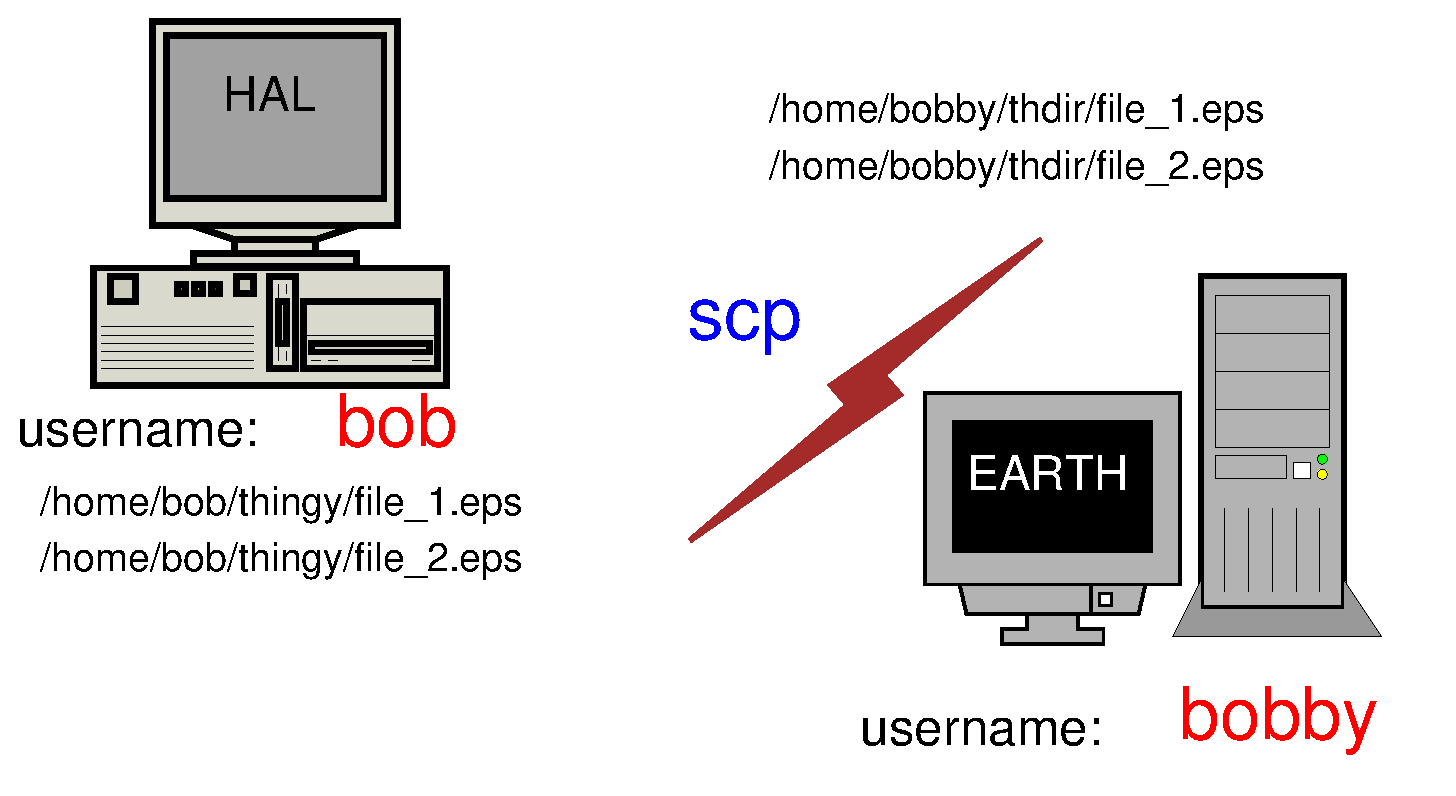
\includegraphics[angle=0,width=5cm]{./Figs/Diagram4.eps}%}
\end{center}
\end{columns}
}
  \end{block}
  
%%%%%%%%%%%%%%%%%%%%%%%%%%%%%%%%%%%%%%%%%%%%%%%%%%%%%%%%%%%%%%%%%%%%%%%%%%%%%%%%%%
\note{
{\tiny

Notes Module V
}
}
\end{frame}
%%%%%%%%%%%%%%%%%%%%%%%%%%%%%%%%%%%%%%%%%%%%%%%%%%%%%%%%%%%%%%%%%%%%%%%%%%%% 
%%%%%%%%%%%%%%%%%%%%%%%%%%%%%%%%%%%%%%%%%%%%%%%%%%%%%%%%%%%%%%%%%%%%%%%%%%%% 
\begin{frame}[t,fragile]{Using \alert{\texttt{scp}} for secure file transfer}
  % ------------------------------------------------------


  \begin{block}{Command syntax: \alert{\texttt{scp} \emph{user1}@\emph{host1:file1}  \emph{user2}@\emph{host2:[file2|dir2]}}}
    {\footnotesize  To transfer from \texttt{hal} to \texttt{earth} the files in the example the syntax is}
{\scriptsize
  \begin{lstlisting}
bob@hal:~$ scp thingy/file_1.eps     bobby@earth:thdir
Password: 
file_1.eps  100%  581     0.6KB/s   00:00    
bob@hal:~$ scp thingy/file_2.eps     bobby@earth:thdir
Password: 
file_2.eps  100%  581     0.6KB/s   00:00    
  \end{lstlisting}
}

{\footnotesize\textbf{(a)}  We have assumed that the remote directory \texttt{thdir} exists. In case it does not exist use the \alert{\texttt{-r}} option. This option also allows the recursive copy of folders and its contents.\\
\textbf{(b)} Wildcards and globbing works in the same way as with the usual \texttt{cp} command.
}

  \end{block}
  
%%%%%%%%%%%%%%%%%%%%%%%%%%%%%%%%%%%%%%%%%%%%%%%%%%%%%%%%%%%%%%%%%%%%%%%%%%%%%%%%%%
\note{
{\tiny

Notes Module V
}
}
\end{frame}
%%%%%%%%%%%%%%%%%%%%%%%%%%%%%%%%%%%%%%%%%%%%%%%%%%%%%%%%%%%%%%%%%%%%%%%%%%%% 
%%%%%%%%%%%%%%%%%%%%%%%%%%%%%%%%%%%%%%%%%%%%%%%%%%%%%%%%%%%%%%%%%%%%%%%%%%%% 
%%%%%%%%%%%%%%%%%%%%%%%%%%%%%%%%%%%%%%%%%%%%%%%%%%%%%%%%%%%%%%%%%%%%%%%%%%%% 
%%%%%%%%%%%%%%%%%%%%%%%%%%%%%%%%%%%%%%%%%%%%%%%%%%%%%%%%%%%%%%%%%%%%%%%%%%%% 
%%%%%%%%%%%%%%%%%%%%%%%%%%%%%%%%%%%%%%%%%%%%%%%%%%%%%%%%%%%%%%%%%%%%%%%%%%%% 
%%%%%%%%%%%%%%%%%%%%%%%%%%%%%%%%%%%%%%%%%%%%%%%%%%%%%%%%%%%%%%%%%%%%%%%%%%%% 
\section{Silent Authentication}
%%%%%%%%%%%%%%%%%%%%%%%%%%%%%%%%%%%%%%%%%%%%%%%%%%%%%%%%%%%%%%%%%%%%%%%%%%%% 
%%%%%%%%%%%%%%%%%%%%%%%%%%%%%%%%%%%%%%%%%%%%%%%%%%%%%%%%%%%%%%%%%%%%%%%%%%%% 
%%%%%%%%%%%%%%%%%%%%%%%%%%%%%%%%%%%%%%%%%%%%%%%%%%%%%%%%%%%%%%%%%%%%%%%%%%%% 
%%%%%%%%%%%%%%%%%%%%%%%%%%%%%%%%%%%%%%%%%%%%%%%%%%%%%%%%%%%%%%%%%%%%%%%%%%%% 
%%%%%%%%%%%%%%%%%%%%%%%%%%%%%%%%%%%%%%%%%%%%%%%%%%%%%%%%%%%%%%%%%%%%%%%%%%%% 
%%%%%%%%%%%%%%%%%%%%%%%%%%%%%%%%%%%%%%%%%%%%%%%%%%%%%%%%%%%%%%%%%%%%%%%%%%%%
\begin{frame}[t,fragile]{Using silent authentication with \alert{\texttt{ssh}} \textbf{(A)}}
  % ------------------------------------------------------
  \vspace{-0.2cm}
  \begin{block}{\textbf{(A)} Generate user's keypair}
    {\footnotesize The creation by a user of a public/private key pair and its exchange
with a remote system allows the user to login silently withouth
password typing for identification. If user \texttt{bob} in \texttt{hal} wants to login silently in \texttt{earth} the steps are the following:}

{\scriptsize
  \begin{lstlisting}
bob@hal:~$ ssh-keygen -t rsa
Generating public/private rsa key pair.
Enter file in which to save the key (/home/bob/.ssh/id_rsa): [ENTER]
Enter passphrase (empty for no passphrase): [ENTER]
Enter same passphrase again: [ENTER] ...
6e:8a:0d:f7:cb:40:7a:3a:0c:31:18:37:35:37:47:f6 bob@hal.local
The key's randomart image is:
+--[ RSA 2048]----+
|   .o o.+        |
|. o  o + .       |
| + .      E      |
|. o              |
|    o.o +.       |
+-----------------+
bob@hal:~$ 
  \end{lstlisting}
}

% {\footnotesize\textbf{(a)}  We have assumed that the remote directory \texttt{thdir} exists. In case it does not exist use the \alert{\texttt{-r}} option. This option also allows the recursive copy of folders and its contents.\\
% \textbf{(b)} Wildcards and globbing works in the same way as with the usual \texttt{cp} command.
% }

  \end{block}
  
%%%%%%%%%%%%%%%%%%%%%%%%%%%%%%%%%%%%%%%%%%%%%%%%%%%%%%%%%%%%%%%%%%%%%%%%%%%%%%%%%%
\note{
{\tiny

Notes Module V
}
}
\end{frame}
%%%%%%%%%%%%%%%%%%%%%%%%%%%%%%%%%%%%%%%%%%%%%%%%%%%%%%%%%%%%%%%%%%%%%%%%%%%% 
%%%%%%%%%%%%%%%%%%%%%%%%%%%%%%%%%%%%%%%%%%%%%%%%%%%%%%%%%%%%%%%%%%%%%%%%%%%%
%%%%%%%%%%%%%%%%%%%%%%%%%%%%%%%%%%%%%%%%%%%%%%%%%%%%%%%%%%%%%%%%%%%%%%%%%%%% 
%%%%%%%%%%%%%%%%%%%%%%%%%%%%%%%%%%%%%%%%%%%%%%%%%%%%%%%%%%%%%%%%%%%%%%%%%%%%
\begin{frame}[t,fragile]{Using silent authentication with \alert{\texttt{ssh}} \textbf{(B)}}
  % ------------------------------------------------------
    {\footnotesize  Two options to copy the public key to the remote \texttt{\textasciitilde/.ssh/authorized\_keys}.}
  \begin{block}{\textbf{(B.1)}  Using \texttt{\alert{ssh-copy-id}} (preferred)}
{\scriptsize
  \begin{lstlisting}
bob@hal:~$ ssh-copy-id -i .ssh/id_rsa.pub bobby@earth
bobby@earth's password: 
Now try logging into the machine, with "ssh 'bobby@earth'", and check in:
  .ssh/authorized_keys
to make sure we haven't added extra keys that you weren't expecting.
  \end{lstlisting}%$
}
  \end{block}
  \begin{block}{\textbf{(B.2)}  Using \texttt{\alert{ssh}}}
{\scriptsize
  \begin{lstlisting}
cat .ssh/id_rsa.pub | ssh bobby@earth "cat >> .ssh/authorized_keys"
\end{lstlisting}
%$
}

  \end{block}
  \begin{block}{\textbf{(B.3)}  Removing a computer from  \texttt{authorized\_keys}}
{\scriptsize
  \begin{lstlisting}
bobby@earth:~$  ssh-keygen -R hal
  \end{lstlisting}
  % $
}

  \end{block}
  
%%%%%%%%%%%%%%%%%%%%%%%%%%%%%%%%%%%%%%%%%%%%%%%%%%%%%%%%%%%%%%%%%%%%%%%%%%%%%%%%%%
\note{
{\tiny

Notes Module V
}
}
\end{frame}
%%%%%%%%%%%%%%%%%%%%%%%%%%%%%%%%%%%%%%%%%%%%%%%%%%%%%%%%%%%%%%%%%%%%%%%%%%%% 
%%%%%%%%%%%%%%%%%%%%%%%%%%%%%%%%%%%%%%%%%%%%%%%%%%%%%%%%%%%%%%%%%%%%%%%%%%%% 